\chapter{Project Management}
\label{chap:final-project-management}

In this chapter, we evaluate the overall project management during the thesis. Indeed, as defined in the initial specifications, the milestones were meant to be adjustable based on the project iterations. Our primary constraint for the Master's Thesis was the time: indeed, the project is formally framed to start on the 17th of September 2019 and end on 7th of February 2020, for a total of amount of 900 hours. To evaluate the project management, we plan three steps; first, we take a high-level overview and comment on the two project phases, the \glsfirst{sota} research and GraphQA as our research contribution. Secondly, we will review and reflect on the initial specification, and finally conclude on the overall management.

\section{High-Level Overview}
Initially defined as \textit{Back to Level} and \textit{Diving into the Subject}, the two phases had the same meaning overall to, what we believe to be, our academic vision defined as Research and Contribution. In this chapter, we take a step back to visualize the entire work done as a whole to summarise the exciting adventure of our first academic research.

\subsection{State-of-the-Art Research}
Our first step to avoid being overwhelmed with knowledge from the most advanced \gls{nlp} papers in the field of \gls{qa} systems and \glspl{gs} was to plan the research.  As we did not have the tools to understand the papers properly, we decided to define a workflow to gather valuable information, such as the initial tools to get started with more complicated techniques. The listing below shows our procedure.

\begin{itemize}
    \setlength\itemsep{0em}
    \item Get up to date with the \gls{nlp} technologies used at our lab, \textit{iCoSys}.
    \item Explore community-made curated lists\footnote{\textit{Awesome} NLP lists from \url{github.com}}.
    \item Subscribe to various specilized social medias to stay informed of the latest \gls{nlp} breakthroughs \footnote{Examples from \url{reddit.com} /r/MachineLearning, /r/LanguageTechnology, /r/deeplearning}.
    \item Read reviews and article summarises of recent papers\footnote{Particularly from community based \url{medium.com} articles}.
    \item Deeply analyse the latest breakthrough papers and read all the mentioned paper.
    \item Filter and read the latest preprints \footnote{Most of the articles are coming from \url{arxiv.com} and \url{aclweb.org}}.
\end{itemize}

Using this workflow, we could in 6 weeks read about 40 papers and gently examine 40 others, which we believe gave us an approximately fair overview of the \gls{nlp} field, and particularly of the \gls{qa} systems and \glspl{gs}.

\subsection{Research Contribution}
Based on the accumulated knowledge from the \gls{sota} research, we could analyze the current techniques used and their applications in the field of \gls{nlp}, in particular, for \gls{qa} systems and \glspl{gs}. Which helped us define a scope for the project that would make sense in the scope of a Master's Thesis to contribute to \gls{nlp}. Gladly, our constraint to use \gls{wikidata} \gls{kb} could sharpen the possible contributions. As stated in our analysis \ref{chap:analysis}, we went through multiple brainstorming and project iterations to get to GraphQA. From a management point of view, it appears that we respected the initial planning and honored the objectives defined in the initial project specification. Finally, we believe that our work could contribute to \gls{nlp}, making the second phase as a success. 


\section{Specification Review}
In this section, we review the original specifications by adding comments as a retrospective approach. We keep the structure and often paraphrase the original content. To improve reading, when content is reused or paraphrased, we set it in \textit{italic} and in \textbf{bold} for comments. Additionally, for use the \checkmark and $\times$ bullets to mark items as realized or not realized.

\subsection{Intrinsic Objectives}
\subsubsection{Primaries}
In this section we presented the tasks that we believed to be essential to get started with the master's thesis. 

\begin{itemize}[noitemsep]
    \item[\checkmark] \textit{Propose a project specification and planning.} %\textbf{We added the initial brainstormed tasks to the annexes.}
    \item[\checkmark] \textit{Analyze the \gls{sota} of existing technologies and technics of \gls{qa} systems and \gls{generative} \gls{ai}.}
    \item[\checkmark] \textit{Overview digital transformation in journalism} \textbf{Even if we did the study, we did not include the search as the project shifted toward chatbots and \gls{nlp}.}
    \item[\checkmark] \textit{Review the current status of the AI-News project.}
    \item[\checkmark] \textit{Document the study and write the thesis.}
\end{itemize}

%\todo{add the annexes numbering to for the brainstormed tasks}

\subsection{Fact-based Question-Answering Chatbot Objectives}
\textit{The first objective is to make, based on the \glsfirst{sota}, an algorithm that takes a question as input and outputs a response, as illustrated on Figure~\ref{fig:management_qa}}

\begin{figure}
    \centering
    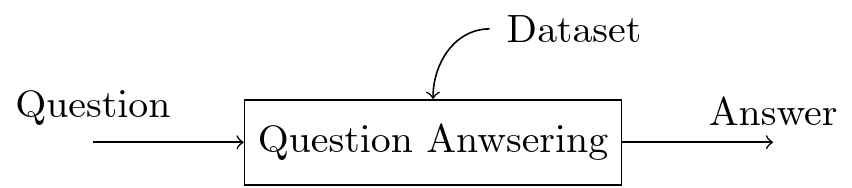
\includegraphics[width=\textwidth,height=2.1cm,keepaspectratio=true]{intro_qa}
    \caption{Suggested \gls{qa} diagram}
    \label{fig:management_qa}
\end{figure}

\subsubsection{Primaries}
\begin{itemize}[noitemsep]
    \item[\checkmark] \textit{Select existing papers and projects treating the subject as a starting point.}
    \item[\checkmark] \textit{Identify relevant datasets.}
    \item[\checkmark] \textit{Develop one or more \gls{poc}.}
    \item[\checkmark] \textit{Test and evaluate solutions.}
    \item[\checkmark] \textit{Suggest improvements, possible continuation, and future outcomes.}
\end{itemize}

\subsubsection{Secondaries}
\begin{itemize}[noitemsep]
    \item[$\times$] \textit{Extend the \gls{qa} chatbot using "tailored" knowledge, e.g., \gls{model-ft} with press content.} \textbf{As mentioned in the final notes from the GraphQA chapter \ref{chap:graphqa}, this item can be extrapolated to GraphQA by adding a fine-tuned pretrain language model for a multi-brains approach to reach a consensus-based answer.}
\end{itemize}

\subsection{Natural Language Question Answering Chatbot Objectives}
\textit{The second objective was to extend the output from the \gls{qa} system, from the first objective, by enhancing the answers and generate human-like sentences from the enhanced answers. The initial vision for this objective is as illustrated in Figure~\ref{fig:planning_qa_gen}, a two parts system. The \textit{Enricher} enriches the answer from the \gls{qa} system, e.g. using a knowledge base\footnote{Wikidata.org, a Freebase-based  \autocite{paper:bollacker2008} knowledge base or Google's Knowledge Graphs \autocite{blog:intro_knowledge_graph}}. The \textit{Generator} aims at creating readable text from the enriched answer. Besides, we could also use user profiles\footnote{Fictive profiles in the context of the thesis} as input to those two parts.}

\begin{figure}[ht!]
    \centering
    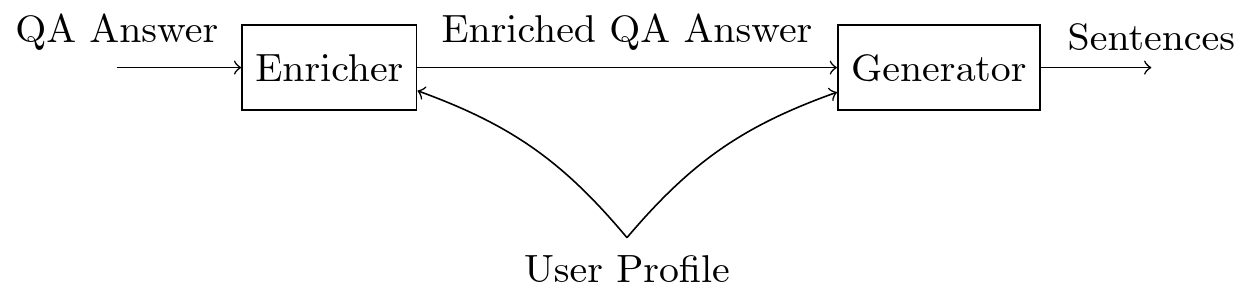
\includegraphics[width=\textwidth,keepaspectratio=true]{intro_qa_gen}
    \caption{Suggested \gls{generative} \gls{qa} diagram}
    \label{fig:planning_qa_gen}
\end{figure}


\paragraph{Primaries}
\begin{itemize}[noitemsep]
    \item[\checkmark] \textit{Investigate a rule-based system for keyword enrichment.}
    \item[\checkmark] \textit{Generate sentences with keywords.}
    \item[\checkmark] \textit{Identify relevant datasets.}
    \item[\checkmark] \textit{Develop one or more \gls{poc}.}
    \item[\checkmark] \textit{Test and evaluate solutions.}
    \item[\checkmark] \textit{Suggest improvements, possible continuation, and future outcomes.}
\end{itemize}

\paragraph{Secondaries}
\begin{itemize}[noitemsep]
    \item[\checkmark] \textit{Use advanced strategies to enrich keywords.}
    \item[\checkmark] \textit{Use advanced text generation technics such as GTP-2\footnote{OpenAI's GTP-2 Algorithm \autocite{papers:gpt2}}.}
    \item[$\times$] \textit{Use user profiles to customize the outputs.} \textbf{This item is mentioned in the final notes from the GraphQA chapter \ref{chap:graphqa}. GraphQA could build long-term context graphs for each user to hold their preferences. It could hold particular interests (entities), injected for the user each time a new Sub-Knowledge Graph is generated. The result would be that GraphQA will try to find a path to the answer using the users injected interests.}
\end{itemize}

\subsection{Objectives Retrospective}
For the objectives, we indeed honored the primary functions and even could add secondary functions to the GraphQA. Even if initial planned, we did not build two distinct \glspl{poc}. Indeed, we started with an hybrid model combining the required features into a single \gls{poc} (see Figure \ref{fig:fig_planning_qa_gen_hybrid}).


\subsection{Methodologies}
\textit{For consistency, the project was separated into two methodological parts. In the first third, as the project targets information gathering and self-study, we used a standard sequential project management methodology. For the next two-thirds of the project, we used an agile methodology to perform incremental progress while exploring.}

\subsubsection{Back to level Milestones}
\textit{First third of the study, from 16.09.19 to 25.10.19 (6 weeks).}
\begin{enumerate}
    \setlength\itemsep{0em}
    \item[\checkmark M1.] \textit{Initial \gls{mt} plan and project specification}
    \item[\checkmark M2.] \textit{Review the \gls{sota} for the \gls{nlp} and \gls{nlu} technologies and refine the plan if needed.}
\end{enumerate}

\subsubsection{Diving into the subject Milestones}
\textit{From 28.10.19 to 07.02.20 (13 weeks), the following two-third of the work is composed of 6 sprints of two weeks each and one week to finalize the thesis.}
\begin{itemize}
    \setlength\itemsep{0em}
    \item[\checkmark M3.] \textit{Basic \gls{qa} Chatbot}
    \item[\checkmark M4.] \textit{Evaluation of basic \gls{qa} Chatbot}
    \item[\checkmark M5.] \textit{Basic generative \gls{qa} Chatbot}
    \item[\checkmark M6.] \textit{Evaluation of basic generative \gls{qa} Chatbot}
\end{itemize}

\subsection{Initial Gantt}
\textit{The Figure~\ref{fig:gantt-initial} represents the chart for the initial plan.}

\subsection{Methologies Retrospective}
The two phases split were respected from a methodological and temporal point of view; however, the objectives hybridization (see Figure \ref{fig:fig_planning_qa_gen_hybrid}) made the milestones slightly altered as the evaluation milestones M4 and M6 are combined. 

\section{Management Conclusion}
We believe that it is important to note that even if the objectives and the results are positives, it is difficult from a management point of view to validate the statement that the end results justify the means, which we think happened in the scope of our master's thesis. Indeed, even if we enjoyed every minute, we did massive overtime for the project to reach our objectives, which means that either the initial project scope or the post-analysis redefined scope was too large for our time constraint. We blame the rescoping as the project shifted toward an understudied field of \gls{nlp} and \gls{qa} systems, which made us notice that we could define a potential new field of the \gls{nlp} research. On a final management note, even if from an industrial point of view, the current overtime would not be easily accepted. In our case; however, from an academic point of view, we justify our overflow as passionate dedication and as a fair attitude to contribute to research.

\subsection{Final Milestones}
\begin{itemize}
    \setlength\itemsep{0em}
    \item[M1.] Initial \gls{mt} plan and project specification
    \item[M2.] Review the \gls{sota} for the \gls{nlp} and \gls{nlu} technologies and refine the plan if needed.
    \item[M3.] GraphQA 1 (see Chapter \ref{graphqa:graphqa1})
    \item[M4.] GraphQA 2 (see Chapter \ref{graphqa:graphqa2})
    \item[M5.] GraphQA 3 (see Chapter \ref{graphqa:graphqa3})
    \item[M6.] Evaluation of basic generative \gls{qa} Chatbot
    \item[M7.] Turn in Master's Thesis
\end{itemize}

\subsection{Effective Gantt}
The Figure~\ref{fig:gantt-final} represents the chart for for the effective plan.

\begin{figure}
    \centering
    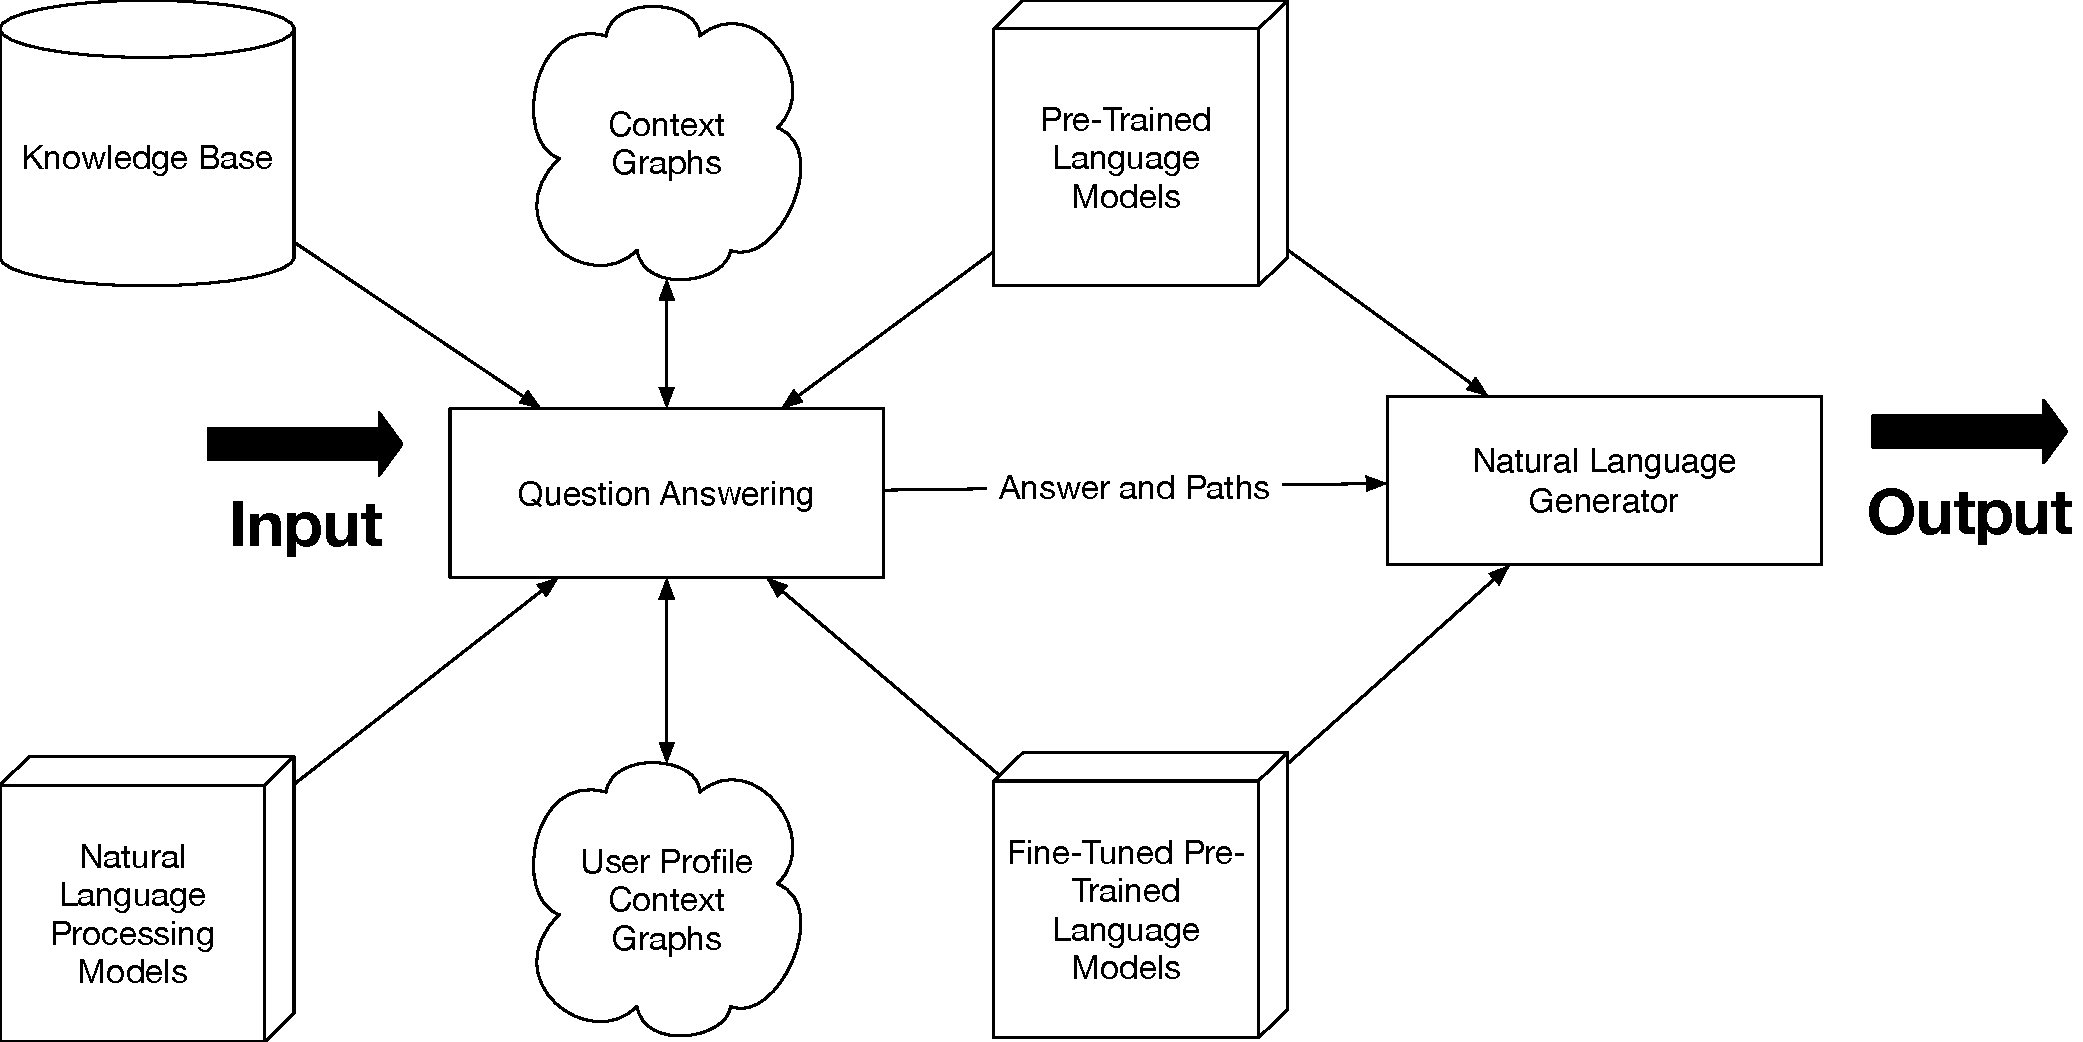
\includegraphics[width=\textwidth,keepaspectratio=true]{fig_planning_qa_gen_hybrid}
    \caption{Suggested \gls{generative} \gls{qa} diagram}
    \label{fig:fig_planning_qa_gen_hybrid}
\end{figure}



\newganttchartelement*{project-milestone}{
project-milestone/.style={
shape=isosceles triangle,
inner sep=0pt,
draw=cyan,
top color=white,
bottom color=cyan!50
},
project-milestone incomplete/.style={
/pgfgantt/project-milestone,
draw=yellow,
bottom color=yellow!50
},
project-milestone label font=\slshape,
project-milestone left shift=0pt,
project-milestone right shift=0pt
}

\newgantttimeslotformat{stardate}{
\def\decomposestardate##1.##2\relax{
\def\stardateyear{##1}\def\stardateday{##2}
}
\decomposestardate#1\relax
\pgfcalendardatetojulian{\stardateyear-01-01}{#2}
\advance#2 by-1\relax
\advance#2 by\stardateday\relax
}

\begin{figure}%[h]%[htbp]
\centering
\begin{ganttchart}[vgrid, hgrid]{1}{19}
\gantttitle{Sep}{2} 
\gantttitle{Oct}{5}
\gantttitle{Nov}{4}
\gantttitle{Dec}{3}
\gantttitle{Jan}{4}
\gantttitle{Feb}{1}\\
\gantttitlelist{1,...,19}{1}\\

%part 1
\ganttgroup{Back to level}{1}{6} \\
\ganttmilestone{M1, M2}{3}
\ganttmilestone{}{6}\\

%part 2
\ganttgroup{Diving}{7}{18} \\
\ganttbar{Sprint 1}{7}{8} \\
\ganttbar{Sprint 2}{9}{10} \\
\ganttmilestone{M3}{10}\\
\ganttbar{Sprint 3}{11}{12} \\
\ganttmilestone{M4}{12}\\
\ganttbar{Sprint 4}{13}{14} \\
\ganttbar{Sprint 5}{15}{16} \\
\ganttmilestone{M5}{16}\\
\ganttbar{Sprint 6}{17}{18} \\
\ganttmilestone{M6}{18}\\

%\ganttlink{elem6}{elem7}
%\ganttlink{elem8}{elem9}

%part 3
\ganttgroup{Wrap up}{19}{19} \\


\end{ganttchart}

\caption{Initial Gantt Chart}
\label{fig:gantt-initial}
\end{figure}


\begin{figure}%[h]%[htbp]
\centering
\begin{ganttchart}[vgrid, hgrid]{1}{19}
\gantttitle{Sep}{2} 
\gantttitle{Oct}{5}
\gantttitle{Nov}{4}
\gantttitle{Dec}{3}
\gantttitle{Jan}{4}
\gantttitle{Feb}{1}\\
\gantttitlelist{1,...,19}{1}\\

%part 1
\ganttgroup{State-of-the-Art Research}{1}{6} \\
\ganttmilestone{M1, M2}{3}
\ganttmilestone{}{6}\\

%part 2
\ganttgroup{Research Contribution}{7}{19} \\
\ganttbar{Sprint 1}{7}{8} \\
\ganttbar{Sprint 2}{9}{10} \\
\ganttmilestone{M3}{10}\\
\ganttbar{Sprint 3}{11}{12} \\
\ganttmilestone{M4}{12}\\
\ganttbar{Sprint 4}{13}{14} \\
\ganttbar{Sprint 5}{15}{16} \\
\ganttmilestone{M5}{16}\\
\ganttbar{Sprint 6}{17}{18} \\
\ganttmilestone{M6}{18}\\
\ganttmilestone{M7}{19}\\

%\ganttlink{elem6}{elem7}
%\ganttlink{elem8}{elem9}

%part 3
\ganttgroup{Writing Thesis}{18}{19} \\

\end{ganttchart}

\caption{Effective Gantt Chart}
\label{fig:gantt-final}
\end{figure}


